\subsection{Agenda}
%%%%%%%%%%%%%%%%%%%%%%%%%%%%%%%%%%%%%%%%%%%%%%%%%%%%%%%%%%%%%%%%%%%%%%%%%%%%%%%%%%%%%%%%%%%%%%%%%%% 
\begin{frame}
	
	 Origins of Advanced Encryption Standard
	 Requirements for AES
	%\item Description of the cipher
	%\item Key Expansion
	%\item Attacks on AES
	
\end{frame}
%%%%%%%%%%%%%%%%%%%%%%%%%%%%%%%%%%%%%%%%%%%%%%%%%%%%%%%%%%%%%%%%%%%%%%%%%%%%%%%%%%%%%%%%%%%%%%%%%%%	

\subsection{AES Origins}
%%%%%%%%%%%%%%%%%%%%%%%%%%%%%%%%%%%%%%%%%%%%%%%%%%%%%%%%%%%%%%%%%%%%%%%%%%%%%%%%%%%%%%%%%%%%%%%%%%% 
\begin{frame}
	\frametitle{Advanced Encryption Standard}
		\framesubtitle{Origins}
	{\footnotesize
	\hspace{0.5cm}{Due to limitations of DES (small key and block sizes), National Institute of Standards and Technology (NIST) started a open process to select a new block cipher. In the 1998, fifteen proposals were submitted.}\\ 
	\vspace{0.2cm}	
	\hspace{0.5cm}{AES is a subset of the Rijndael cipher developed by two Belgian cryptographers, Vincent Rijmen and Joan Daemen, who submitted a proposal to NIST during the AES selection process. It supersedes the Data Encryption Standard (DES).}\\
	\vspace{0.2cm}
	\hspace{0.5cm}{AES is available in many different encryption packages, and is the first (and only) publicly accessible cipher approved by the National Security Agency (NSA) for top secret information.}\\
	}
\end{frame}
%%%%%%%%%%%%%%%%%%%%%%%%%%%%%%%%%%%%%%%%%%%%%%%%%%%%%%%%%%%%%%%%%%%%%%%%%%%%%%%%%%%%%%%%%%%%%%%%%%%

\subsection{Requirements for AES} 
%%%%%%%%%%%%%%%%%%%%%%%%%%%%%%%%%%%%%%%%%%%%%%%%%%%%%%%%%%%%%%%%%%%%%%%%%%%%%%%%%%%%%%%%%%%%%%%%%%%
\begin{frame}
	\frametitle{Advanced Encryption Standard}
		\framesubtitle{Requirements for AES}
		In the selection process, NIST asked for: \\
		{\footnotesize 
		\hspace{0.5cm}{- A block cipher, block length: 128 bit}\\
		\hspace{0.5cm}{- Key length: 128, 192 and 256 bit}\\
		\hspace{0.5cm}{- Suitability for hardware and software}\\
		}
		\vspace{0.2cm}
		{\normalsize NIST platform used to test candidate cipher algorithms:}\\
		{\footnotesize
		\hspace{0.5cm}{- PC IBM-compatible,Pentium Pro 200 MHz, 64 MB RAM, WINDOWS 95}\\
		\hspace{0.5cm}{- Borland C++ 5.0 compiler and Java Development Kit (JDK) 1.1}\\
		}
		\vspace{0.2cm}
		{\normalsize NIST selection of the winning algorithm based on:}\\
		{\footnotesize
		\hspace{0.5cm}{- Security}\\
		\hspace{0.5cm}{- Efficient implementation \textbf{both} in hardware and software}\\
		\hspace{0.5cm}{- Code length and memory utilization}\\
		}	
\end{frame}
%%%%%%%%%%%%%%%%%%%%%%%%%%%%%%%%%%%%%%%%%%%%%%%%%%%%%%%%%%%%%%%%%%%%%%%%%%%%%%%%%%%%%%%%%%%%%%%%%%%

\subsection{AES overwiev} 
%%%%%%%%%%%%%%%%%%%%%%%%%%%%%%%%%%%%%%%%%%%%%%%%%%%%%%%%%%%%%%%%%%%%%%%%%%%%%%%%%%%%%%%%%%%%%%%%%%%
\begin{frame}
	\frametitle{Advanced Encryption Standard}
		\framesubtitle{Overwiev of AES}
	{\normalsize 	
	\hspace{0.5cm}{• AES is \textbf{not} Feistel Network}\\
	\hspace{0.5cm}{• AES is a type of substitution-permutation network}\\
    \hspace{0.5cm}{• AES has 128 bits block size}\\
    \hspace{0.5cm}{• AES has three allowable key sizes K: 128,192,256 bit }\\
    \hspace{0.5cm}{• AES has variable number of rounds:}\\
	}
	{\footnotesize
	\hspace{1.0cm}{- If K= 128, then Nr= 10}\\
	\hspace{1.0cm}{- If K= 192, then Nr= 12}\\
	\hspace{1.0cm}{- If K= 256, then Nr= 14}\\
	}
\end{frame}
%%%%%%%%%%%%%%%%%%%%%%%%%%%%%%%%%%%%%%%%%%%%%%%%%%%%%%%%%%%%%%%%%%%%%%%%%%%%%%%%%%%%%%%%%%%%%%%%%%%

\subsection{Algorithm}
%%%%%%%%%%%%%%%%%%%%%%%%%%%%%%%%%%%%%%%%%%%%%%%%%%%%%%%%%%%%%%%%%%%%%%%%%%%%%%%%%%%%%%%%%%%%%%%%%%%
\begin{frame}
	\frametitle{Advanced Encryption Standard}
		\framesubtitle{Key and Block}	
	{\normalsize
	{ \textbf{Key} with variable length (128, 192, 256 bits), represented with a matrix (array) of bytes with 4 \textit{rows}
	and $N_k$ \textit{columns},}\\ 
	{$N_k$ = key length/32:}\\
    \hspace{0.5cm}{– Key of 128 bits = 16 bytes, $N_k$ = 4}\\
    \hspace{0.5cm}{– Key of 192 bits = 24 bytes, $N_k$ = 6}\\
    \hspace{0.5cm}{– Key of 256 bits = 32 bytes, $N_k$ = 8}\\
	\vspace{0.2cm}
{\textbf{Block} length 128 bits, represented with a matrix (array) of bytes with 4 \textit{rows} and $N_b$ \textit{columns}, $N_b$ = block length/32:}\\
	\hspace{0.5cm}{– Block of 128 bits = 16 bytes, $N_b$ = 4}\\
	
	}

\end{frame}
%%%%%%%%%%%%%%%%%%%%%%%%%%%%%%%%%%%%%%%%%%%%%%%%%%%%%%%%%%%%%%%%%%%%%%%%%%%%%%%%%%%%%%%%%%%%%%%%%%%

%%%%%%%%%%%%%%%%%%%%%%%%%%%%%%%%%%%%%%%%%%%%%%%%%%%%%%%%%%%%%%%%%%%%%%%%%%%%%%%%%%%%%%%%%%%%%%%%%%%
\begin{frame}
	\frametitle{Advanced Encryption Standard}
		\framesubtitle{State}	
		{\normalsize Internally, the AES algorithm’s operations are performed on a two-dimensional array of bytes called the \textbf{State}  \\
		\hspace{0.5cm}{- Four rows, each containing Nb bytes}\\
		\hspace{0.5cm}{- Nb columns, constituted by 32-bit words}\\
		\hspace{0.5cm}{- Sr,c denotes the byte in row \textit{r} and column \textit{c}}\\	
		\hspace{0.5cm}{- The array of bytes in input is copied in the State matrix}\\
		\hspace{0.5cm}{- At the end, the State matrix is copied in the output matrix}\\	
		}	
\end{frame}
%%%%%%%%%%%%%%%%%%%%%%%%%%%%%%%%%%%%%%%%%%%%%%%%%%%%%%%%%%%%%%%%%%%%%%%%%%%%%%%%%%%%%%%%%%%%%%%%%%%

%%%%%%%%%%%%%%%%%%%%%%%%%%%%%%%%%%%%%%%%%%%%%%%%%%%%%%%%%%%%%%%%%%%%%%%%%%%%%%%%%%%%%%%%%%%%%%%%%%%
\begin{frame}
	\frametitle{Advanced Encryption Standard}
		\framesubtitle{Steps for encryption}
	\vspace{-0.2cm}
	\begin{figure}
		\centering
		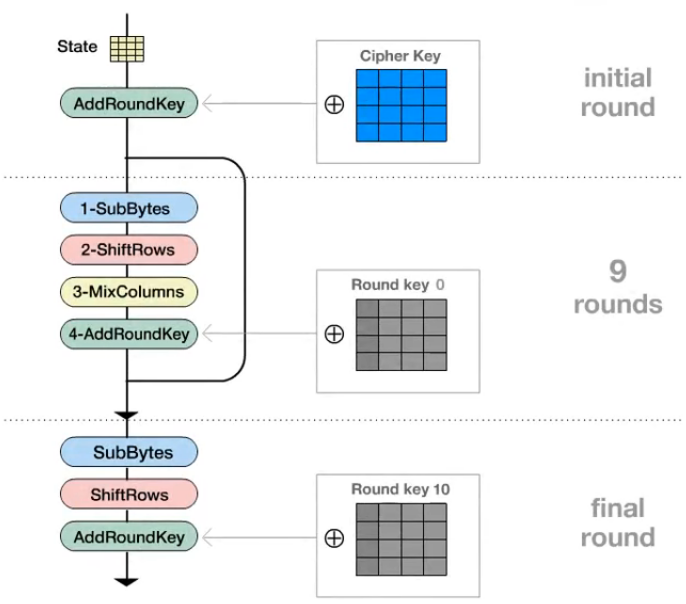
\includegraphics[width=7cm]{encryption}
		\caption{AES algorithm description}
		\label{fig:obrazek encryption}
	\end{figure}
\end{frame}
%%%%%%%%%%%%%%%%%%%%%%%%%%%%%%%%%%%%%%%%%%%%%%%%%%%%%%%%%%%%%%%%%%%%%%%%%%%%%%%%%%%%%%%%%%%%%%%%%%%	

%%%%%%%%%%%%%%%%%%%%%%%%%%%%%%%%%%%%%%%%%%%%%%%%%%%%%%%%%%%%%%%%%%%%%%%%%%%%%%%%%%%%%%%%%%%%%%%%%%%
\begin{frame}
	\frametitle{Advanced Encryption Standard}
		\framesubtitle{1.SubBytes}
	{\normalsize 	
	{• Byte substitution using a non-linear (but \textit{invertible}) S-Box (independently on each byte)}\\
	{• S-box is represented as a 16x16 array, rows and columns indexed by hexadecimal bits}\\
    {• 8 bytes replaced as follows: 8 bytes define a hexadecimal number \textbf{rc}, then $S_{r,c}$ = binary(S-box(r,c))}\\
    \vspace{0.4cm}
    {• How is AES S-box different from DES S-boxes?}\\
	\hspace{0.5cm}{- Only \underline{\textbf{one}} S-box}\\
	\hspace{0.5cm}{- S-boxes based on modular arithmetic with polynomials, can be}\\
	\hspace{0.4cm}{defined algebraically}\\
	\hspace{0.5cm}{- Easy to analyze, prove attacks fail}\\
	}
\end{frame}
%%%%%%%%%%%%%%%%%%%%%%%%%%%%%%%%%%%%%%%%%%%%%%%%%%%%%%%%%%%%%%%%%%%%%%%%%%%%%%%%%%%%%%%%%%%%%%%%%%%

%%%%%%%%%%%%%%%%%%%%%%%%%%%%%%%%%%%%%%%%%%%%%%%%%%%%%%%%%%%%%%%%%%%%%%%%%%%%%%%%%%%%%%%%%%%%%%%%%%%
\begin{frame}
	\frametitle{Advanced Encryption Standard}
		\framesubtitle{1.SubBytes using Rijndael S-Box Table}
	\vspace{0.5cm}
		\begin{figure}
		\centering
		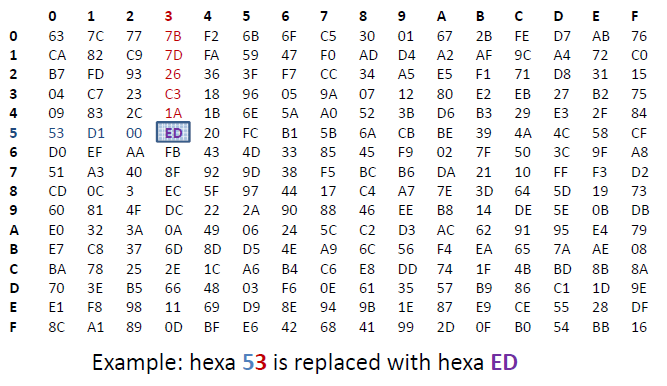
\includegraphics[width=10cm]{sbox}
		\label{fig:obrazek sbox}
	\end{figure}
\end{frame}
%%%%%%%%%%%%%%%%%%%%%%%%%%%%%%%%%%%%%%%%%%%%%%%%%%%%%%%%%%%%%%%%%%%%%%%%%%%%%%%%%%%%%%%%%%%%%%%%%%%

%%%%%%%%%%%%%%%%%%%%%%%%%%%%%%%%%%%%%%%%%%%%%%%%%%%%%%%%%%%%%%%%%%%%%%%%%%%%%%%%%%%%%%%%%%%%%%%%%%%
\begin{frame}
	\frametitle{Advanced Encryption Standard}
		\framesubtitle{2.ShiftRows}
	\vfill
	\vspace{-0.5cm}
	\begin{block}{}
\footnotesize {The first row is left unchanged. Each byte of the second row is shifted one to the left. Similarly, the third and fourth rows are shifted by offsets of two and three respectively.}
	\end{block}
		\begin{figure}
		\centering
		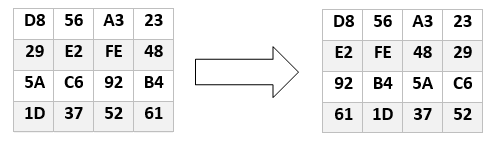
\includegraphics[width=8cm]{shiftrows}
		%\caption{basic elements of AES algorithm}
		\label{fig:obrazek sbox}
	\end{figure}
\end{frame}
%%%%%%%%%%%%%%%%%%%%%%%%%%%%%%%%%%%%%%%%%%%%%%%%%%%%%%%%%%%%%%%%%%%%%%%%%%%%%%%%%%%%%%%%%%%%%%%%%%%

%%%%%%%%%%%%%%%%%%%%%%%%%%%%%%%%%%%%%%%%%%%%%%%%%%%%%%%%%%%%%%%%%%%%%%%%%%%%%%%%%%%%%%%%%%%%%%%%%%%
\begin{frame}
	\frametitle{Advanced Encryption Standard}
		\framesubtitle{3.MixColumns}
		\vfill
	\vspace{-1cm}
	\begin{block}{}
		\footnotesize {
    	{Each column is represented as a 4 byte vector.}\\
		{Each column of State is replaced by a new column which is formed by multiplying that column by a certain 			matrix of elements of the field.}\\
    	{We can also see this operation as polynomial multiplication where each column is represented with 				 	polynomial a(x):}\\
		\hspace{0.5cm}{$a(x) = c(x).a(x) mod x^{4}+1= ({03}x^3 + {01}x^2 + {01}x + {02})
.(a_3x^3 + a_2x^2 + a_1x^1 + a_0) mod x^4 + 1 $}\\
		}
	\end{block}
	\begin{block}{}
	{ $$c(x)= \left[
        \begin{array}{cccc}
         02 & 03 & 01 & 01\\
         01 & 02 & 03 & 01\\
         01 & 01 & 02 & 03\\
         03 & 01 & 01 & 02
         \end{array}
      \right] $$}
	\end{block}
	
\end{frame}
%%%%%%%%%%%%%%%%%%%%%%%%%%%%%%%%%%%%%%%%%%%%%%%%%%%%%%%%%%%%%%%%%%%%%%%%%%%%%%%%%%%%%%%%%%%%%%%%%%%

%%%%%%%%%%%%%%%%%%%%%%%%%%%%%%%%%%%%%%%%%%%%%%%%%%%%%%%%%%%%%%%%%%%%%%%%%%%%%%%%%%%%%%%%%%%%%%%%%%%
\begin{frame}
	\frametitle{Advanced Encryption Standard}
		\framesubtitle{3.MixColumns }
		\vfill
		\begin{figure}
		\centering
		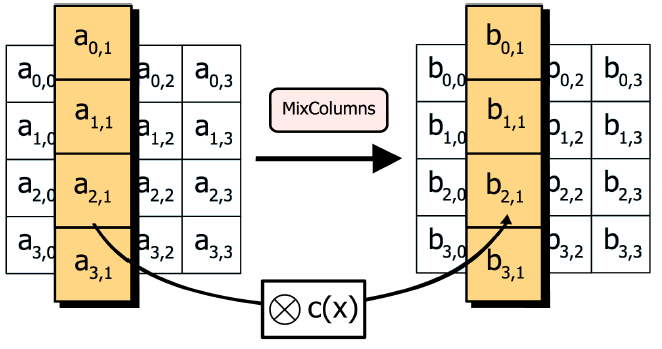
\includegraphics[width=10cm]{mixcolumn}
		\label{fig:obrazek mixcolumn}
	\end{figure}
\end{frame}
%%%%%%%%%%%%%%%%%%%%%%%%%%%%%%%%%%%%%%%%%%%%%%%%%%%%%%%%%%%%%%%%%%%%%%%%%%%%%%%%%%%%%%%%%%%%%%%%%%%

%%%%%%%%%%%%%%%%%%%%%%%%%%%%%%%%%%%%%%%%%%%%%%%%%%%%%%%%%%%%%%%%%%%%%%%%%%%%%%%%%%%%%%%%%%%%%%%%%%%
\begin{frame}
	\frametitle{Advanced Encryption Standard}
		\framesubtitle{4.AddRoundKey}
	\vfill
	\vspace{-0.5cm}
	\begin{block}{}
\footnotesize {The subkey is added by combining each byte of the state with the corresponding byte of the subkey using bitwise XOR.}
	\end{block}
	%\vspace{0.5cm}
		\begin{figure}
		\centering
		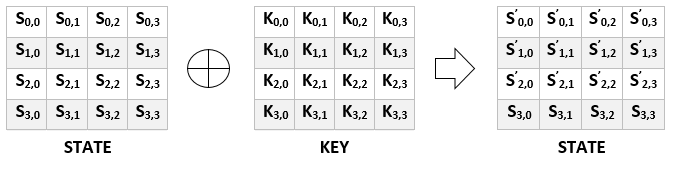
\includegraphics[width=10cm]{addroundkey}
		%\caption{basic elements of AES algorithm}
		\label{fig:obrazek addroundkey}
	\end{figure}
\end{frame}
%%%%%%%%%%%%%%%%%%%%%%%%%%%%%%%%%%%%%%%%%%%%%%%%%%%%%%%%%%%%%%%%%%%%%%%%%%%%%%%%%%%%%%%%%%%%%%%%%%%
\subsection{Key} % Change, please!
%%%%%%%%%%%%%%%%%%%%%%%%%%%%%%%%%%%%%%%%%%%%%%%%%%%%%%%%%%%%%%%%%%%%%%%%%%%%%%%%%%%%%%%%%%%%%%%%%%%
\begin{frame}
	\frametitle{Advanced Encryption Standard}
		\framesubtitle{Key Schedule}
		\vspace{-2cm}
		\begin{block}{}
		{\normalsize
	Since the key schedule for 128-bit, 192-bit, and 256-bit encryption are very similar, with only some constants changed, the following keysize constants are defined here:}\\
	{\footnotesize
	\hspace{0.5cm}{• $n$ has a value of 16 for 128-bit keys, 24 for 192-bit keys, and 32 for 256-bit}\\ 
	\hspace{0.7cm}{keys}\\
	\hspace{0.5cm}{• $b$ has a value of 176 for 128-bit keys, 208 for 192-bit keys, and 240 for}\\ 
	\hspace{0.7cm}{256-bit keys (with 128-bit blocks as in AES, it is correspondingly larger}\\ 
	\hspace{0.7cm}{for variants of Rijndael with larger block sizes).}
	}
	\end{block}
\end{frame}
%%%%%%%%%%%%%%%%%%%%%%%%%%%%%%%%%%%%%%%%%%%%%%%%%%%%%%%%%%%%%%%%%%%%%%%%%%%%%%%%%%%%%%%%%%%%%%%%%%%

%%%%%%%%%%%%%%%%%%%%%%%%%%%%%%%%%%%%%%%%%%%%%%%%%%%%%%%%%%%%%%%%%%%%%%%%%%%%%%%%%%%%%%%%%%%%%%%%%%%
\begin{frame}
	\frametitle{Advanced Encryption Standard}
		\framesubtitle{Key Schedule: Rcon}
		{\normalsize
		\hspace{0.5cm}Rcon is what the Rijndael documentation calls the exponentiation of 2 to a user-specified value. Note that this operation 	is not performed with regular integers, but in Rijndael's finite field. In polynomial form, 2 is:
		\vspace{0.2cm}
		\begin{block}{}
	$2_{10}=00000010_2=0x^7+0x^6+0x^5+0x^4+0x^3+0x^2+1x+0x=b $,\\
	\end{block}
	{and we compute:}\\
	\begin{block}{}
	$rcon(i)=2^{i-1}=2*2^{i-2}=2*rcon(i-1)$\\
	\end{block}
	}
\end{frame}
%%%%%%%%%%%%%%%%%%%%%%%%%%%%%%%%%%%%%%%%%%%%%%%%%%%%%%%%%%%%%%%%%%%%%%%%%%%%%%%%%%%%%%%%%%%%%%%%%%%

%%%%%%%%%%%%%%%%%%%%%%%%%%%%%%%%%%%%%%%%%%%%%%%%%%%%%%%%%%%%%%%%%%%%%%%%%%%%%%%%%%%%%%%%%%%%%%%%%%%
\begin{frame}

	\frametitle{Advanced Encryption Standard}
	\framesubtitle{Expanding 128-bit key}
	\vspace{-0.5cm}
	{\scriptsize
    {1.The first 16 bytes of the expanded key are simply the encryption key}\\
    {2.The rcon iteration value i is set to 1}\\
    {3.Until we have 176 bytes of expanded key, we do the following to generate 16 more bytes of expanded key:}\\
    \hspace{0.4cm}{1.We do the following to create the first four bytes of expanded key:}\\
    \hspace{0.8cm}{1.We create a 4-byte temporary variable, t}\\
    \hspace{0.8cm}{2.We assign the value of the previous four bytes in the temporary key to t}\\
    \hspace{0.8cm}{3.We rotate one byte to te left}\\
    \hspace{0.8cm}{4.We substitute bytes on t with Rijndael S-Box}\\
    \hspace{0.8cm}{5.We XOR t with i as the rcon iteration value.}\\
    \hspace{0.8cm}{6.We increment i by one.}\\
    \hspace{0.8cm}{7.We XOR t with the first four-bytes of the old key.}\\
    \hspace{0.8cm}{This becomes the next four bytes in the expanded key.}\\
    \hspace{0.4cm}{2.We then do the following three times to create the next twelve bytes of expanded}\\
    \hspace{0.4cm}{key:}\\
    \hspace{0.8cm}{1.We assign the value of the previous four bytes in the temporary key to t}\\
    \hspace{0.8cm}{2.We XOR t with the four-byte block 16 bytes before the new expanded key.}\\ 
    \hspace{0.8cm}{This becomes the next four bytes in the expanded key.} \\
    {4.Done. We now have 176 bytes of key generated.}\\
	}
	
\end{frame}
%%%%%%%%%%%%%%%%%%%%%%%%%%%%%%%%%%%%%%%%%%%%%%%%%%%%%%%%%%%%%%%%%%%%%%%%%%%%%%%%%%%%%%%%%%%%%%%%%%%

\subsection{Attacks on AES} 
%%%%%%%%%%%%%%%%%%%%%%%%%%%%%%%%%%%%%%%%%%%%%%%%%%%%%%%%%%%%%%%%%%%%%%%%%%%%%%%%%%%%%%%%%%%%%%%%%%%
\begin{frame}
	\frametitle{Advanced Encryption Standard}
		\framesubtitle{Attacks on AES}
		{\normalsize
		\textbf{Algebraic attacks}\\
		\vspace{0.4cm}
		{People have shown Rijndael can be written as an over defined system of multivariate quadratic equations.}\\ 
		{Paper published at Eurocrypt 2000 Shamir describe an algorithm called XL able to solve efficiently many such systems of 					equations.}\\
		\begin{alertblock}{}
		{However this fails miserably!}\\
		\end{alertblock}
		{The problem of recovering the secret key from one single plaintext can be written as a system of 8000 quadratic equations with 1600 binary unknowns.}\\
		}
\end{frame}
%%%%%%%%%%%%%%%%%%%%%%%%%%%%%%%%%%%%%%%%%%%%%%%%%%%%%%%%%%%%%%%%%%%%%%%%%%%%%%%%%%%%%%%%%%%%%%%%%%%

%%%%%%%%%%%%%%%%%%%%%%%%%%%%%%%%%%%%%%%%%%%%%%%%%%%%%%%%%%%%%%%%%%%%%%%%%%%%%%%%%%%%%%%%%%%%%%%%%%%
\begin{frame}
	\frametitle{Advanced Encryption Standard}
		\framesubtitle{Attacks on AES}
		\vspace{-2cm}
		{\normalsize
		\textbf{Algebraic attacks(cont.)}\\
		\vspace{0.4cm}
		{Nicolas Courtois and Josef Pieprzyk investigate how to improve XL and adapt it to such special systems. They propose a new class 		of attacks, attack, called XSL attacks.}\\ 
		\vspace{0.4cm}
		{Ciphers like Rijndael were referred to as XSL ciphers, because their rounds are composed of the XOR of key material, a nonlinear 		substitution provided by an S-box, and a linear diffusion stage.} 
		}
\end{frame}
%%%%%%%%%%%%%%%%%%%%%%%%%%%%%%%%%%%%%%%%%%%%%%%%%%%%%%%%%%%%%%%%%%%%%%%%%%%%%%%%%%%%%%%%%%%%%%%%%%%

%%%%%%%%%%%%%%%%%%%%%%%%%%%%%%%%%%%%%%%%%%%%%%%%%%%%%%%%%%%%%%%%%%%%%%%%%%%%%%%%%%%%%%%%%%%%%%%%%%%
\begin{frame}
	\frametitle{Advanced Encryption Standard}
		\framesubtitle{Attacks on AES}
 		{\normalsize
		\textbf{Theory that breaks AES-128 }\\
		{In 2011, Andriej Bogdanow, Dymitr Kowratowicz and Christian Rechberger devise a theoretical way to broke any cipher that is using 		AES-128}\\
		{Despite the fact, it was impractical. It would take billions of years. This is an example:}\\
		}
		\begin{block}{}
		{\footnotesize
		{If you assume:}\\
		\hspace{0.5cm}{- Every person on the planet owns 10 computers.}\\
		\hspace{0.5cm}{- There are 7 billion people on the planet.}\\
		\hspace{0.5cm}{- Each of these computers can test 1 billion key combinations per second.}\\
    	\hspace{0.5cm}{- On average, you can crack the key after testing half of the possibilities.}\\
    	\vspace{0.2cm}
    	{Then the earth's population can crack one encryption key in 77,000,000,000,000,000,000,000,000 years!}\\
		}
		\end{block}
\end{frame}
%%%%%%%%%%%%%%%%%%%%%%%%%%%%%%%%%%%%%%%%%%%%%%%%%%%%%%%%%%%%%%%%%%%%%%%%%%%%%%%%%%%%%%%%%%%%%%%%%%%
	
%%%%%%%%%%%%%%%%%%%%%%%%%%%%%%%%%%%%%%%%%%%%%%%%%%%%%%%%%%%%%%%%%%%%%%%%%%%%%%%%%%%%%%%%%%%%%%%%%%%
\begin{frame}
\frametitle{Advanced Encryption Standard}
	\framesubtitle{Attacks on AES}
	\begin{center}
		\Huge \textbf{Is the AES secure?}
	\end{center}

\end{frame}
%%%%%%%%%%%%%%%%%%%%%%%%%%%%%%%%%%%%%%%%%%%%%%%%%%%%%%%%%%%%%%%%%%%%%%%%%%%%%%%%%%%%%%%%%%%%%%%%%%%

%%%%%%%%%%%%%%%%%%%%%%%%%%%%%%%%%%%%%%%%%%%%%%%%%%%%%%%%%%%%%%%%%%%%%%%%%%%%%%%%%%%%%%%%%%%%%%%%%%%
\begin{frame}
	\frametitle{Advanced Encryption Standard}
		\framesubtitle{Attacks on AES}
		\vspace{-1cm}
 		{\normalsize
		\textbf{AES-256 keys sniffed in seconds }\\
		}
		{\footnotesize
		\hspace{0.4cm}{Researchers at Fox‑IT have managed to wirelessly extract secret AES-256 encryption keys from a distance of one 				metre, using \$200 worth of parts obtained from a standard electronics store}\\
		\hspace{0.4cm}{The research team used a simple loop antenna, attached it to an external amplifier and bandpass filters bought 				online, and then plugged it into a software defined radio USB stick they bought for \$20.}\\
		\hspace{0.4cm}{By running a different encryption run on a test rig, the researchers mapped out how the power consumption related 			to individual bytes of information. That allowed them to take guesses at the 256 possible values of a single byte and the 					correct choice showed the highest power spike.}\\
		\hspace{0.4cm}{There are, of course, some caveats. The tests took place under laboratory conditions, rather than in a busy office 		or server room where other signals might interfere with the data collection. But it's an interesting example of how an attack 				previously thought of as unfeasible due to cost and distance has been made easier by smarter and cheaper technology.}\\		
		}
\end{frame}
%%%%%%%%%%%%%%%%%%%%%%%%%%%%%%%%%%%%%%%%%%%%%%%%%%%%%%%%%%%%%%%%%%%%%%%%%%%%%%%%%%%%%%%%%%%%%%%%%%%

%%%%%%%%%%%%%%%%%%%%%%%%%%%%%%%%%%%%%%%%%%%%%%%%%%%%%%%%%%%%%%%%%%%%%%%%%%%%%%%%%%%%%%%%%%%%%%%%%%%
\begin{frame}
	
	\begin{center}
		\Huge \textbf{Thank you for attention!}
	\end{center}

\end{frame}
%%%%%%%%%%%%%%%%%%%%%%%%%%%%%%%%%%%%%%%%%%%%%%%%%%%%%%%%%%%%%%%%%%%%%%%%%%%%%%%%%%%%%%%%%%%%%%%%%%%